% Closed-loop form v3: the argument, as a superposition table. NOT a loop diagram.
% v1 asserted the equality in a label; v2 drew it as a rewiring of four loop diagrams. Both
% keep the plant on the page, which is self-defeating for a figure whose message is that the
% plant is not involved: you cannot show an absence by drawing the thing four times. A block
% diagram also shows TOPOLOGY, while this argument is arithmetic on SIGNALS, and in a block
% diagram a signal is a line, which has no identity.
% v3 therefore contains no plant and no loop at all. Three signals, one operator applied to
% each, and the same relation on both sides of the box. The absence IS the argument.
% Keep v2: it shows what is implemented. v3 shows why it is valid. Different jobs.
% Style: figure-style.md, notation from the closed-loop table in README.
% Compile: pdflatex closed-loop-form-v3.tex
\documentclass[border=12pt]{standalone}
\usepackage{tikz}
\usetikzlibrary{arrows.meta, calc}
\usepackage{amsmath}

\begin{document}
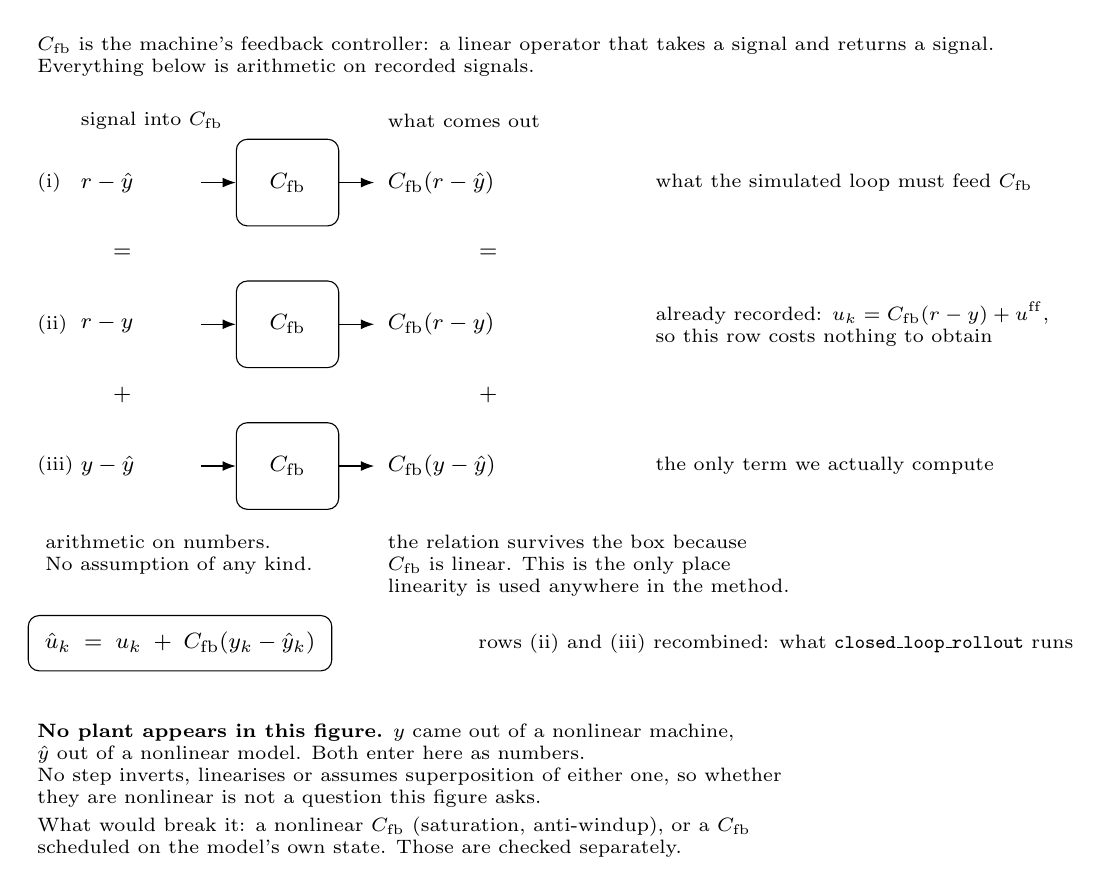
\begin{tikzpicture}[>=Latex, font=\footnotesize,
  block/.style={draw, rounded corners, minimum width=26mm, minimum height=12mm, align=center},
  rblock/.style={draw, rounded corners, minimum width=13mm, minimum height=11mm, align=center},
  small/.style={draw, rounded corners, minimum width=15mm, minimum height=10mm, align=center},
  sum/.style={draw, circle, minimum size=7mm, inner sep=0pt},
  jn/.style={circle, fill, minimum size=3pt, inner sep=0pt}]

\node[anchor=west, align=left, font=\scriptsize] at (0,1.60)
  {$C_{\mathrm{fb}}$ is the machine's feedback controller: a linear operator that takes a signal
   and returns a signal.\\
   Everything below is arithmetic on recorded signals.};

\node[anchor=west, font=\scriptsize] at (0.55,0.78) {signal into $C_{\mathrm{fb}}$};
\node[anchor=west, font=\scriptsize] at (4.45,0.78) {what comes out};

% ---- the three rows -------------------------------------------------------------
\node[anchor=west] at (0,0)     {\scriptsize (i)};
\node[anchor=west] at (0.55,0)  {$r-\hat y$};
\node[rblock] (b1) at (3.30,0)  {$C_{\mathrm{fb}}$};
\draw[->] (2.20,0) -- (b1.west);
\draw[->] (b1.east) -- (4.40,0);
\node[anchor=west] at (4.45,0)  {$C_{\mathrm{fb}}(r-\hat y)$};

\node[anchor=west] at (0,-1.80)    {\scriptsize (ii)};
\node[anchor=west] at (0.55,-1.80) {$r-y$};
\node[rblock] (b2) at (3.30,-1.80) {$C_{\mathrm{fb}}$};
\draw[->] (2.20,-1.80) -- (b2.west);
\draw[->] (b2.east) -- (4.40,-1.80);
\node[anchor=west] at (4.45,-1.80) {$C_{\mathrm{fb}}(r-y)$};

\node[anchor=west] at (0,-3.60)    {\scriptsize (iii)};
\node[anchor=west] at (0.55,-3.60) {$y-\hat y$};
\node[rblock] (b3) at (3.30,-3.60) {$C_{\mathrm{fb}}$};
\draw[->] (2.20,-3.60) -- (b3.west);
\draw[->] (b3.east) -- (4.40,-3.60);
\node[anchor=west] at (4.45,-3.60) {$C_{\mathrm{fb}}(y-\hat y)$};

% ---- the SAME relation, stacked, on both sides of the box ------------------------
\node at (1.20,-0.90) {$=$};
\node at (1.20,-2.70) {$+$};
\node at (5.85,-0.90) {$=$};
\node at (5.85,-2.70) {$+$};

% ---- what each side costs --------------------------------------------------------
\node[anchor=north west, align=left, font=\scriptsize] at (0.10,-4.35)
  {arithmetic on numbers.\\No assumption of any kind.};
\node[anchor=north west, align=left, font=\scriptsize] at (4.45,-4.35)
  {the relation survives the box because\\
   $C_{\mathrm{fb}}$ is linear. This is the only place\\
   linearity is used anywhere in the method.};

% ---- per-row annotations ---------------------------------------------------------
\node[anchor=west, font=\scriptsize] at (7.85,0)
  {what the simulated loop must feed $C_{\mathrm{fb}}$};
\node[anchor=west, align=left, font=\scriptsize] at (7.85,-1.80)
  {already recorded: $u_k=C_{\mathrm{fb}}(r-y)+u^{\mathrm{ff}}$,\\
   so this row costs nothing to obtain};
\node[anchor=west, font=\scriptsize] at (7.85,-3.60)
  {the only term we actually compute};

% ---- the result ------------------------------------------------------------------
\node[draw, rounded corners, inner sep=6pt, anchor=west] at (0,-5.85)
  {$\hat u_k \;=\; u_k \;+\; C_{\mathrm{fb}}(y_k-\hat y_k)$};
\node[anchor=west, font=\scriptsize] at (5.60,-5.85)
  {rows (ii) and (iii) recombined: what \texttt{closed\_loop\_rollout} runs};

% ---- the point -------------------------------------------------------------------
\node[anchor=north west, align=left, font=\scriptsize] at (0,-6.75)
  {\textbf{No plant appears in this figure.} $y$ came out of a nonlinear machine,\\
   $\hat y$ out of a nonlinear model. Both enter here as numbers.\\
   No step inverts, linearises or assumes superposition of either one, so whether\\
   they are nonlinear is not a question this figure asks.\\[2pt]
   What would break it: a nonlinear $C_{\mathrm{fb}}$ (saturation, anti-windup), or a
   $C_{\mathrm{fb}}$\\
   scheduled on the model's own state. Those are checked separately.};

\end{tikzpicture}
\end{document}
